\chapter{Methodology}
\label{ch:methodology}

% Chapter introduction, without a separate section:
% - Formulate the suppression problem, available measurements, admissible stimulation,
%   and the role of a learned Predictor in MPC.
% - Introduce the investigated choices: waveform versus spectral prediction, training
%   objectives, and continuous versus pulse-based stimulation.
% - Explain how these choices connect and introduce the chapter's order.
% Editorial boundary: Chapter 3 supplies general theory. This chapter formulates the
% methods and motivates design choices. Chapter 5 tests them and reports the evidence.
% Introduce tunable parameters and selection criteria here; put search ranges, budgets,
% results, and selected configurations in Chapter 5. Routine tuning can go in an appendix.

\section{Closed-Loop Neurostimulation Architecture}

% i don't like this whole first paragraph. Feels too much like AI
Chapter~\ref{ch:foundations} introduced the plant, electrical interfaces, prediction
models, and receding-horizon control separately. This section connects them into the
closed-loop setting used in this thesis. The setting follows the EEG-feedback structure
of Yu et al.~\cite{Yu2024}, but replaces their amplitude trigger with a prediction model % we don't need to mention what controller they used. This should be in the introduction not here.
and \ac{mpc}. Figure~\ref{fig:closed_loop_architecture} shows the resulting signal path.
Only scalp \ac{eeg} and previously applied electrode currents enter the controller.
The regional activity retained to assess seizure propagation is not available for feedback.

At a controller update, the signal-conditioning stage passes the latest causal % its not "causal signal conditioning" its a low pass filter.
measurement to the prediction model. The \ac{mpc} problem evaluates candidate current
sequences and applies the first current vector of its solution. A zero-order hold keeps
this vector constant until the next update. The stimulation projection converts the
electrode currents into regional membrane perturbations, after which the plant evolves
and produces the next measurement. Waveform and spectral controllers use this same
physical loop. Their update rates differ because a waveform sample is available after
each decimation interval, whereas a spectral quantity is available only after a new
analysis frame has been formed.

\begin{figure}[htbp]
    \centering
    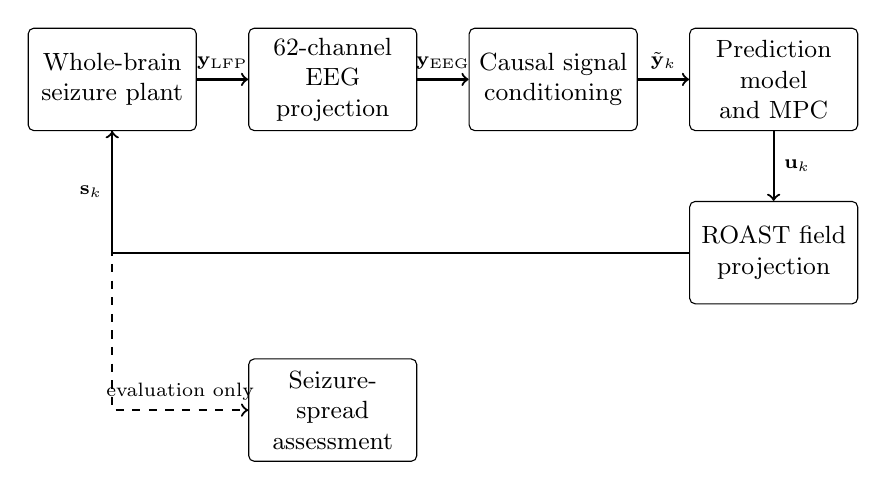
\begin{tikzpicture}[
        block/.style={
            draw,
            rounded corners=2pt,
            align=center,
            minimum height=1.3cm,
            text width=1.9cm,
            font=\small
        },
        signal/.style={->, thick},
        evaluation/.style={->, dashed, thick}
    ]
        \node[block] (plant) at (0,4.2) {Whole-brain seizure plant};
        \node[block] (eeg) at (2.8,4.2) {62-channel EEG projection};
        \node[block] (conditioning) at (5.6,4.2) {Causal signal conditioning};
        \node[block] (control) at (8.4,4.2) {Prediction model and MPC};
        \node[block] (field) at (8.4,2.0) {ROAST field projection};
        \node[block] (assessment) at (2.8,0) {Seizure-spread assessment};

        \draw[signal] (plant) -- node[above, font=\scriptsize] {$\mathbf{y}_\mathrm{LFP}$} (eeg);
        \draw[signal] (eeg) -- node[above, font=\scriptsize] {$\mathbf{y}_\mathrm{EEG}$} (conditioning);
        \draw[signal] (conditioning) -- node[above, font=\scriptsize] {$\tilde{\mathbf{y}}_k$} (control); % is tilde what we use for denoting estimates/filtered values?
        \draw[signal] (control) -- node[right, font=\scriptsize] {$\mathbf{u}_k$} (field);
        \draw[signal] (field) -- (0,2.0) -- node[left, font=\scriptsize] {$\mathbf{s}_k$} (plant);
        \draw[evaluation] (plant) -- (0,0) -- node[above, font=\scriptsize] {evaluation only} (assessment);
    \end{tikzpicture}
    \caption{Closed-loop neurostimulation architecture. Solid arrows denote the causal
        feedback loop. The dashed branch carries regional activity used only for post hoc
        evaluation and does not provide the controller with source-level information.}
    \label{fig:closed_loop_architecture}  %  I don't like this picture. It should show the blocks in a standard closed-loop control block diagram layout. With the EEG projection and ROAST field projection just being multiplication blocks and holding their matrix symbols. There needs to be a "reference"/goal. The seizure spread assessment is not a part of it at all
\end{figure}

\subsection{Plant Configuration and Seizure Dynamics}

The loop in Figure~\ref{fig:closed_loop_architecture} is closed around the biophysical
model of Section~\ref{sec:excitability}. Its plant contains 76 Jansen--Rit regions coupled
by the structural weights and tract lengths of the connectome. Each region contributes  % what connectome? mention that it is the TVB ...
six states, so the instantaneous neural-mass state has dimension 456. Fibre lengths are  % the neural-mass state is irrelevant information. This should just be a description of our setup and what decision we took.
converted into delays using the uniform conduction speed
$c=\SI{50}{\milli\metre\per\milli\second}$, and each delay is rounded to the nearest plant
integration step.

The regional seizure configuration adopts the temporal-lobe partition of Yu et.\.al.~\cite{Yu2024}. % and why is that partition important?
The left hippocampus, left parahippocampal cortex, and left amygdala form  % we need to explain why these regions were chosen.
the \ac{ez}, with $A_i=\SI{3.6}{\milli\volt}$. The left inferior temporal cortex and left
ventral temporal cortex form the initial \ac{pz}, with
$A_i=\SI{3.4}{\milli\volt}$. All remaining regions use the background value
$A_i=\SI{3.25}{\milli\volt}$. The global coupling factor $K=0.60$ and noise intensity
$\sigma=\SI{280}{\per\second}$ were calibrated jointly because both parameters affect the
time at which activity escapes the \ac{ez} and recruits the \ac{pz}. The calibration
criterion rewards early recruitment within the \ac{ez}, later recruitment of the \ac{pz}
and left hemisphere, and little recruitment of the right hemisphere. The calibration
results are reserved for the appendix.

Each simulation starts from the settled healthy state and advances the stochastic delayed
dynamics with the Heun method at $\Delta t=\SI{0.1}{\milli\second}$. One Gaussian increment
is used in both stages of a step. For a standard normal random vector
$\boldsymbol{\xi}_k$, the stochastic increment on the excitatory loop is therefore
$\sigma\sqrt{\Delta t}\,\boldsymbol{\xi}_k$. This fine grid resolves the neural-mass
dynamics and conduction delays. It is not the sampling grid presented to the controller.

\subsection{EEG Measurement and Stimulation Geometry}

The plant configuration fixes the internal seizure dynamics, while closing the loop
requires separate maps for measurement and stimulation. For measurement, the surface
projection supplied with The Virtual Brain maps 16,384 cortical vertices to 62 scalp
electrodes~\cite{SanzLeon2015}. Summing the columns belonging to each anatomical region
reduces this operator from $62\times16{,}384$ to the regional lead field
$\mathbf{L}_\mathrm{EEG}\in\mathbb{R}^{62\times76}$. Equation~\eqref{eq:eeg} then maps the
76 regional \acp{lfp} to the measured scalp signals. No additional measurement noise is
added. Stochastic variability enters through the plant noise described above.

The regional neural-mass output is only proportional to a dipole moment, and neither this
proportionality nor the lead-field data establish an absolute voltage scale. Consequently,
the simulated scalp \ac{eeg} is stated in arbitrary amplitude units. Thresholds and healthy
references are constructed from signals produced by the same forward model, so their
relative scale remains consistent.

The stimulation interface uses the TP9--CP5--Ex8 montage. It extends the CP5--Ex8
placement used by Yu et al.~\cite{Yu2024} with TP9 as a second controllable scalp site.
Ex8 is the return position below the inion defined in the 10--05 cap. During field
generation, ROAST substituted its TPP9 position for the requested TP9 label because this
was the nearest available cap position. The thesis retains TP9 as the requested montage
label and records the substitution here.

ROAST computes one electric-field basis solution for a \SI{1}{\milli\ampere} current at
each controllable scalp electrode against Ex8 on the MNI152 head model~\cite{Huang2019}.
Linear superposition gives the field for any balanced current vector. Let
$\mathbf{E}_{p,i}$ denote the field at the centroid of region $i$ due to the basis current
at electrode $p$, and let $\mathbf{n}_i$ be the outward cortical normal assigned to that
region. The regional membrane perturbation is
%
\begin{equation}
    s_i(t)
    = \lambda_\mathrm{p}\sum_{p=1}^{3}u_p(t)\,
      \mathbf{E}_{p,i}^{\mathsf{T}}\mathbf{n}_i,
    \qquad
    \lambda_\mathrm{p}=\SI{0.35}{\milli\metre} \, .
    \label{eq:regional_stimulation_projection}
\end{equation}
%
The current $u_p$ belongs to electrode $p$, and $\lambda_\mathrm{p}$ is the assumed somatic
polarisation length. The projection in~\eqref{eq:regional_stimulation_projection} uses a
value within the range measured for deep-layer
pyramidal cells~\cite{Radman2009}. Since
$\mathbf{E}_{p,i}^{\mathsf{T}}\mathbf{n}_i$ has units of volts per metre, equivalently
millivolts per millimetre, $s_i$ has units of millivolts. It enters the pyramidal sigmoid as
specified in Section~\ref{sec:electro}. The controller imposes
$|u_p|\leq\SI{2}{\milli\ampere}$ and $\sum_{p=1}^{3}u_p=0$. No slew-rate constraint is used.

The transpose of $\mathbf{L}_\mathrm{EEG}$ cannot supply this stimulation map. Reciprocity
applies when measurement and stimulation use the same electrodes, source locations, and
orientations~\cite{Malmivuo1995}. Ex8 is absent from the 62-channel recording montage, and
the ROAST map samples a volumetric electric field along regional cortical normals. These
conditions differ from those used to construct the \ac{eeg} forward operator.

\subsection{Filtering and Sampling}

The spatial projections determine which signals the controller can measure and apply;
filtering determines which temporal content reaches it. In the simulated seizure regime,
the dominant oscillation lies near \SIrange{3}{4}{\hertz}, and most seizure-related power
lies below \SI{12}{\hertz}, as illustrated in Figure~\ref{fig:bifurcation}. The controller input is
therefore sampled at \SI{50}{\hertz}, retaining frequencies up to the
\SI{25}{\hertz} Nyquist limit while reducing the number of prediction steps.

Before decimation from the \SI{10}{\kilo\hertz} plant grid, every \ac{eeg} channel passes
through a causal fourth-order Butterworth low-pass filter with a \SI{25}{\hertz} cutoff.
A causal filter is required because future samples are unavailable during feedback; a
zero-phase offline filter would give the controller non-causal information. The filtered
signal is then decimated by 200, producing one waveform sample every
\SI{20}{\milli\second}. The same filtering and decimation are applied to identification
data and during closed-loop operation.

The \SI{25}{\hertz} cutoff defines the anti-aliasing stage, not the frequency range used by
a later spectral cost or prediction representation. A waveform controller may update on
the \SI{20}{\milli\second} sample grid. A spectral controller instead updates when its next
causal analysis frame becomes available, so its interval also depends on the frame hop.
Section~\ref{sec:prediction_representations} next defines these two prediction
representations and their time grids.

\section{Prediction Representations and Models}
\label{sec:prediction_representations}
% Motivate the central question: what should be predicted to support seizure suppression?
% Separate the output representation from the model class used to predict its dynamics.

\subsection{Waveform Prediction}
% Define the future EEG waveform to be predicted, the measured history, and the past
% and candidate future currents conditioning the prediction. Motivate this representation.

\subsection{Spectral Observable Prediction}
% Define the spectral Observable and why it is a candidate alternative to waveform prediction. The reason is: if we are only predicting
% Refer to Chapter 3 for STFT theory; specify the representation used in this method.
% Introduce Segment length, Frame hop, frequency selection, pooling, and normalization.
% Explain which information each geometry choice retains or discards and its time scale.
% Keep geometry parameterized here; its empirical selection belongs in Chapter 5.
% QUESTION: Is geometry selected for prediction accuracy, closed-loop suppression,
% temporal responsiveness, or an explicit tradeoff? Define "optimal" relative to that goal.

\subsection{Predictor Model Classes}
% Define the shared autoregressive input-output formulation and multi-step Rollout.
% Introduce the nonlinear MLP and linear/DMD variants and their modeling assumptions.
% Relate DMD to the Koopman perspective only as far as needed to motivate the chosen model.
% Explain which model classes are studied for each representation and why.
% Describe initialization from measured history only to establish a valid prediction.

\section{Predictor Training and Selection}
% Explain how the prediction tasks become identification problems and how candidates
% are selected. This section defines procedures; Chapter 5 reports their outcomes.

\subsection{Identification Data and Prediction Task}
% Describe simulated training data, seizure regimes, and stimulation used to identify
% the response to currents rather than only autonomous dynamics.
% Define history/target construction, prediction duration, and normalization.
% Explain separation of training, selection, and final evaluation data at trajectory level.
% Put experimental dataset sizes and scenario-specific settings in Chapter 5.

\subsection{Waveform and Spectral Training Losses}
% Formulate waveform error, spectral error, and the combinations to be investigated.
% Distinguish a spectral Loss on predicted waveforms from prediction of spectral Observables.
% For the former, STFT geometry defines error scoring; for the latter, it defines the target.
% Introduce the Loss geometry, weights, and scored Spans without claiming selected values.
% QUESTION: Should these two STFT geometries be selected independently, and what must
% remain comparable when evaluating the resulting Predictors?

\subsection{Training Strategies and Selection Criteria}
% Describe fitting procedures and curriculum strategies that are part of the investigation.
% Define the criterion used to select geometry, Loss settings, and model configurations.
% QUESTION: Which choices are scientific comparisons and which are routine tuning?
% QUESTION: Is selection based on open-loop prediction or closed-loop control performance?
% Chapter 5: give search spaces/budgets, compare outcomes, and justify the configurations
% carried into later experiments. Reserve independent evaluation data for final comparisons.

\section{MPC Objectives and Continuous Stimulation}
% Turn the trained Predictor into a controller by defining the optimization problem.

\subsection{Decision Variables and Control Constraints}
% Define the Control Horizon, candidate electrode currents, and predicted dynamics.
% Specify Kirchhoff's law and the Control Budget imposed in the study.
% State the current parameterization and how prediction and control time grids relate.

\subsection{Seizure-Suppression Costs}
% Formulate waveform-based and spectral suppression Costs and their intended behavior.
% Explain construction of the healthy spectral reference and normalization of Cost terms.
% Keep the controller's suppression Cost distinct from the Predictor's training Loss
% and from the post hoc Closed-Loop Evaluation Score used in Chapter 5.

\subsection{Stimulation Penalties}
% Define L2 and L1 current penalties, weight scaling, and the behavior to be compared.
% Describe the smooth L1 surrogate where it is used in the evaluated method.
% End with the complete continuous optimization problem, collecting dynamics, Costs,
% and constraints before extending the formulation to pulses.

\subsection{Numerical Solution and Receding-Horizon Application}
% Explain the transcriptions and solution methods studied, including single/multiple
% shooting and NARX/PCMS formulations if retained as part of the investigation.
% State how Costs spanning multiple samples or Frames enter the optimization.
% Avoid a software architecture account.
% Chapter 5 contains solver comparison protocols and results, not first definitions.

\section{Pulse-Based Control}
% Formulate pulse-based stimulation as an alternative to continuous stimulation.
% Reuse the continuous problem's Predictor, suppression Cost, and current constraints.

\subsection{Pulse Definition and Scheduling Variables}
% Define a pulse before introducing its decision variables and admissible schedules.
% QUESTION: Is the objective to restrict current magnitude, total stimulation time,
% the number of distinct pulses, or some stated combination?
% QUESTION: Does a binary variable denote an active interval or a pulse onset?
% Summing active steps counts enabled intervals; consecutive enabled steps can form one pulse.
% QUESTION: Are pulse shape, duration, polarity, and electrode pattern fixed?
% Which of amplitude, duration/duty cycle, and timing should be optimized?

\subsection{Mixed-Integer Formulation}
% Couple binary scheduling decisions to admissible currents and define the pulse budget.
% State which decisions are shared across electrodes and which are electrode-specific.
% Derive the resulting optimization class from the chosen Predictor, Cost, and constraints.
% Explain the solution approach and any schedule simplifications needed for tractability.
% QUESTION: What is the smallest pulse formulation that tests the intended idea before
% adding amplitude or duty-cycle optimization?

\subsection{Continuous Relaxation and Schedule Recovery}
% Define a relaxation of binary activation variables and how a deliverable schedule
% would be recovered. Explain how feasibility and predicted suppression would be rechecked.
% QUESTION: Which recovery rule preserves the chosen pulse budget and current constraints?
% Distinguish this procedure from continuous optimization of pulse onset times.

\subsection{Continuous Pulse-Timing Alternative}
% Formulate onset times as continuous decisions (if this alternative remains in scope)
% Explain how candidate pulses occurring within a sampling interval affect prediction.
% Develope a continuous-time Predictor required
% Compare the formulations conceptually with L2/L1 continuous stimulation here.
% Chapter 5 compares their suppression, stimulation use, and computational cost.
